\documentclass[letterpaper,12pt]{article}
\usepackage[utf8]{inputenc}
\usepackage{graphicx}
\usepackage{amssymb,amsmath}
\usepackage{verbatim}
\usepackage[parfill]{parskip}
\usepackage{hyperref}
\usepackage{listings}
\usepackage{pdfpages}
\usepackage{longtable}

\title{Information Retrieval CS 834 : Assignment 5}
\author{Miranda Smith\\ msmit213@odu.edu}
\begin{document}
\maketitle
\date{}

\begin{abstract}
Exercise questions 10.3, 10.5, 10.6, 10.11, 11.5 completed. Spring 2017. 
\end{abstract}

\pagebreak

\section{Problem 10.3}
 Compute five iterations of HITS (see Algorithm 3) and PageRank (see Figure 4.11) on the graph in Figure 10.3. Discuss how the PageRank scores compare to the hub and authority scores produced by HITS.

\subsection{Solution}
I calculated the HITS and page rank score by hand and with excel 103.xlsx  got the following results. I did it by hand instead of programming it or using a library so I could better understand how the formulas were working. I did not include iterations 1-3 because they are included in the book and mine are identical.

\begin{center}
Iteration 4
\begin{tabular}{ |c|c|c|c| } 
 \hline
 Node & Hub & Auth & PageRank \\ 
 \hline
 1 & 0.14 & 0.24 & 0.03 \\ 
 \hline
 2 &0  & 0.32 &0.05\\ 
 \hline
 3 & 0.45 &  0 &0.02\\ 
 \hline
 4 &0  &  0.44&0.06\\ 
 \hline
 5 & 0.21 & 0 &0.02\\ 
 \hline
 6 & 0.21 & 0 &0.02\\ 
 \hline
 7 & 0 & 0 &0.02\\ 
 \hline
\end{tabular}
\end{center}

\begin{center}
Iteration 5
\begin{tabular}{ |c|c|c|c| } 
 \hline
 Node & Hub & Auth & PageRank \\ 
 \hline
 1 & 0.15 & 0.24 & 0.03 \\ 
 \hline
 2 &0  & 0.31 &0.05\\ 
 \hline
 3 & 0.45 &  0 &0.02\\ 
 \hline
 4 &0  &  0.45&0.06\\ 
 \hline
 5 & 0.2 & 0 &0.02\\ 
 \hline
 6 & 0.2 & 0 &0.02\\ 
 \hline
 7 & 0 & 0 &0.02\\ 
 \hline
\end{tabular}
\end{center}

Page Rank only needed 3 iterations to converge to a number. The numbers are a lot lower and it seems to be harser than HITS. For example Node 3 ended up with a hub score of 0.45, the highest of all 7 but its page rank is 0.02, one of the lowest. Page rank doesn't take into consideration the importance of being a hub and ranks them without consideration to a page pointing to good pages.
\pagebreak

\section{Problem 10.5}
Find a community-based question answering site on the Web and ask two questions, one that is low-quality and one that is high-quality. Describe the answer
quality of each question.

\subsection{Solution}

I chose stackoverflow because it is theQ \& A website I am most familiar with. I chose two questions that I had come across and had difficulty solving in a different class information visualization that have value as a question and only varied the quality with which I asked the question. These questions focus on programming with d3. It is the hope that the similar post time of the question and the similar topics would make the results of the questions as similar as possible in regard to the people who might have answered and remove as much bias as possible.

\subsubsection{High quality question}
I created this question by taking two graphs in d3 to be displayed on the same page and broke it by naming the variables the same instead of renaming everything. I included all the code that I had written and highlighted the important parts and what I had tried as thoroughly as possble, but left out explicitly mentioning the few extra variables I needed to rename to fix it.
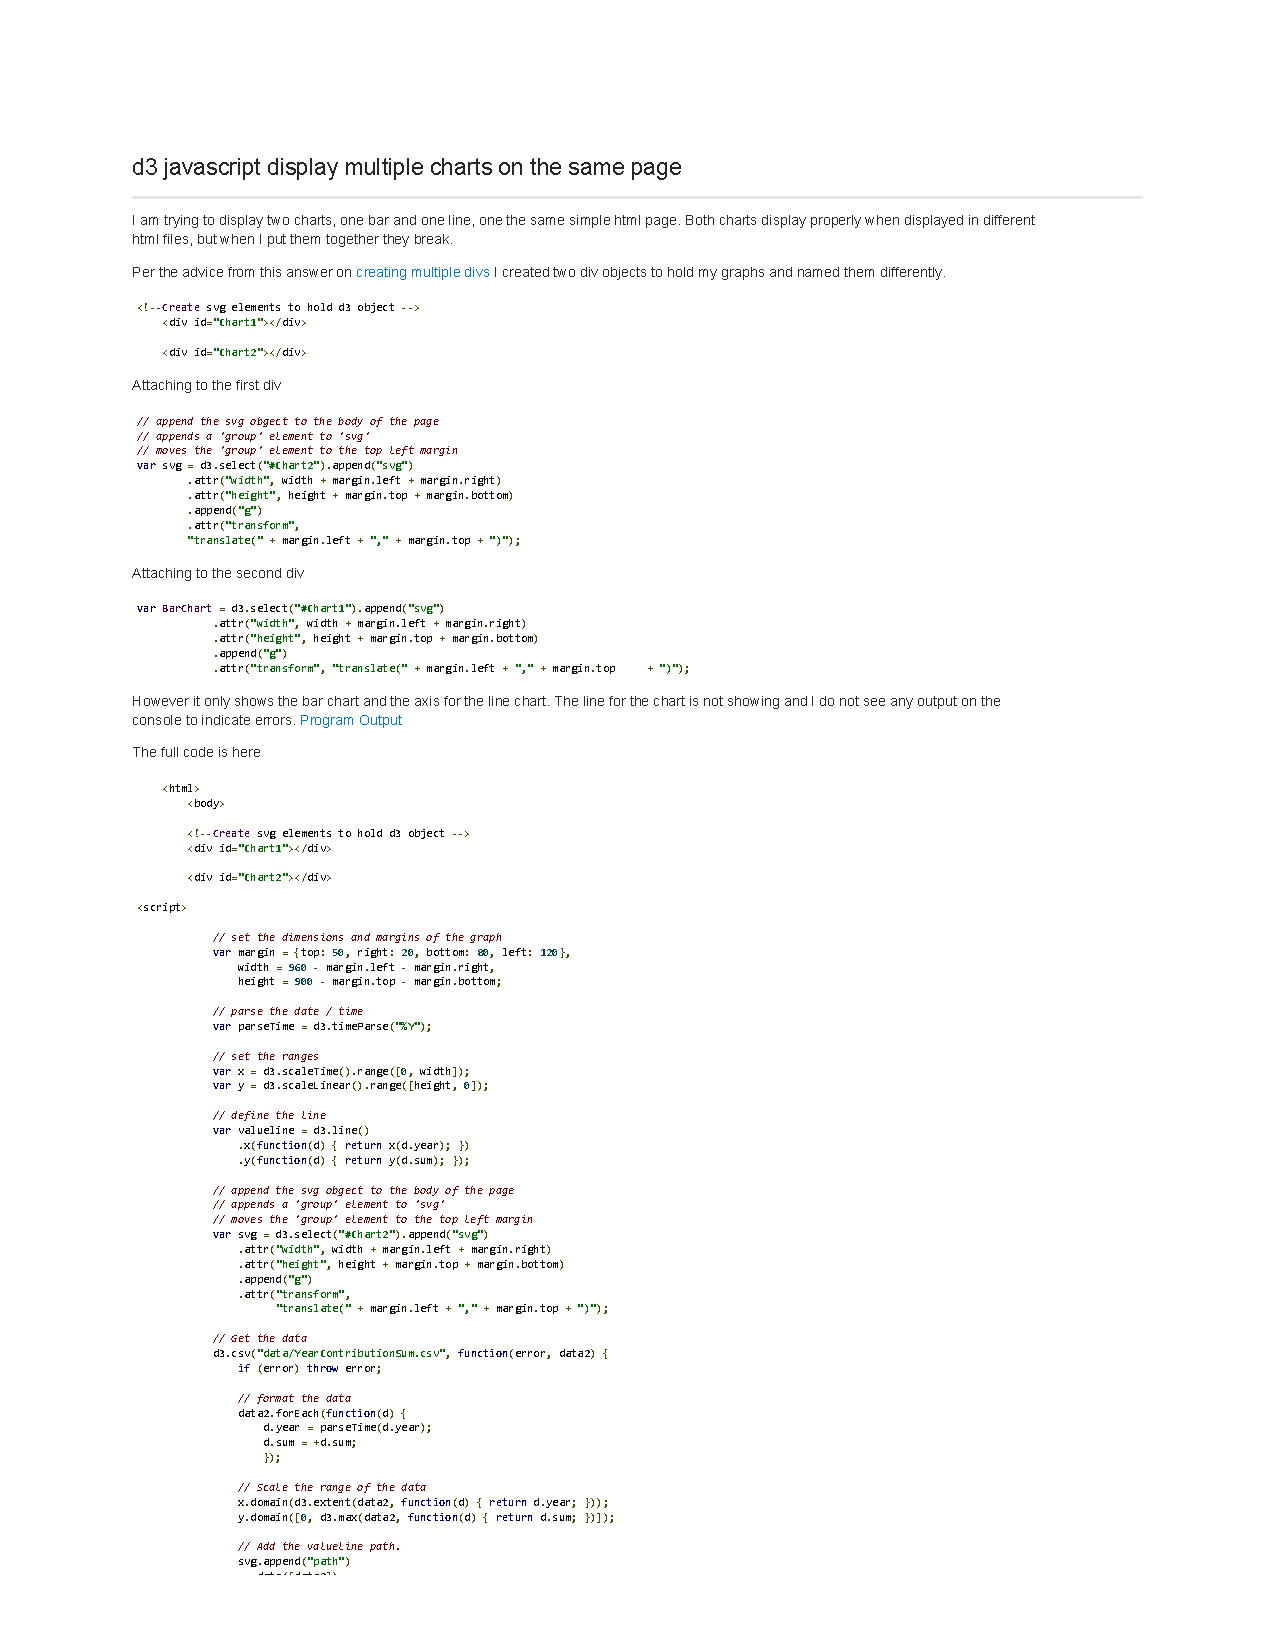
\includepdf[pages={1-}]{105highquality.pdf}

I had two people respond. The first comment came very close to fixing the issue, they only thing missing was changing the margin along with the axis. The offical answer given doesn't change what I was expecting them to but they created a JSbin shown in figure \ref{highQ} and got the code working for me and created mock data to give it since I didn't include that. They seemed to have put a lot of effort into the answer.

\begin{figure}[h]
  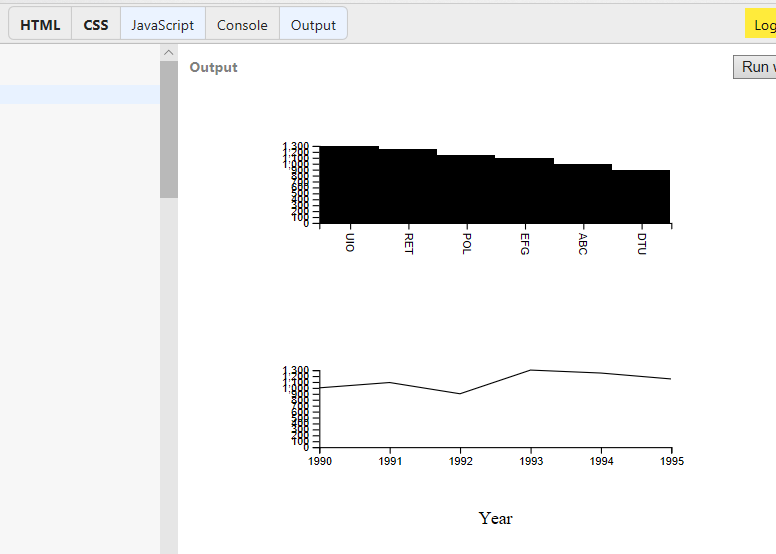
\includegraphics[width=\linewidth]{105highanswer.PNG}
  \caption{Solution Provided}
  \label{highQ}
\end{figure}

\subsubsection{Low quality question}
This question I asked in an ad hoc manner. I proveded the minimum amout of effort to get my question across but still had a valid good quality question to be asked. I chose to interpret low quality to mean the effort put into the question and not that its meaning was indecipherable. I provided no code that I had written, only linked to a page showing an example of a grouped bar chart.
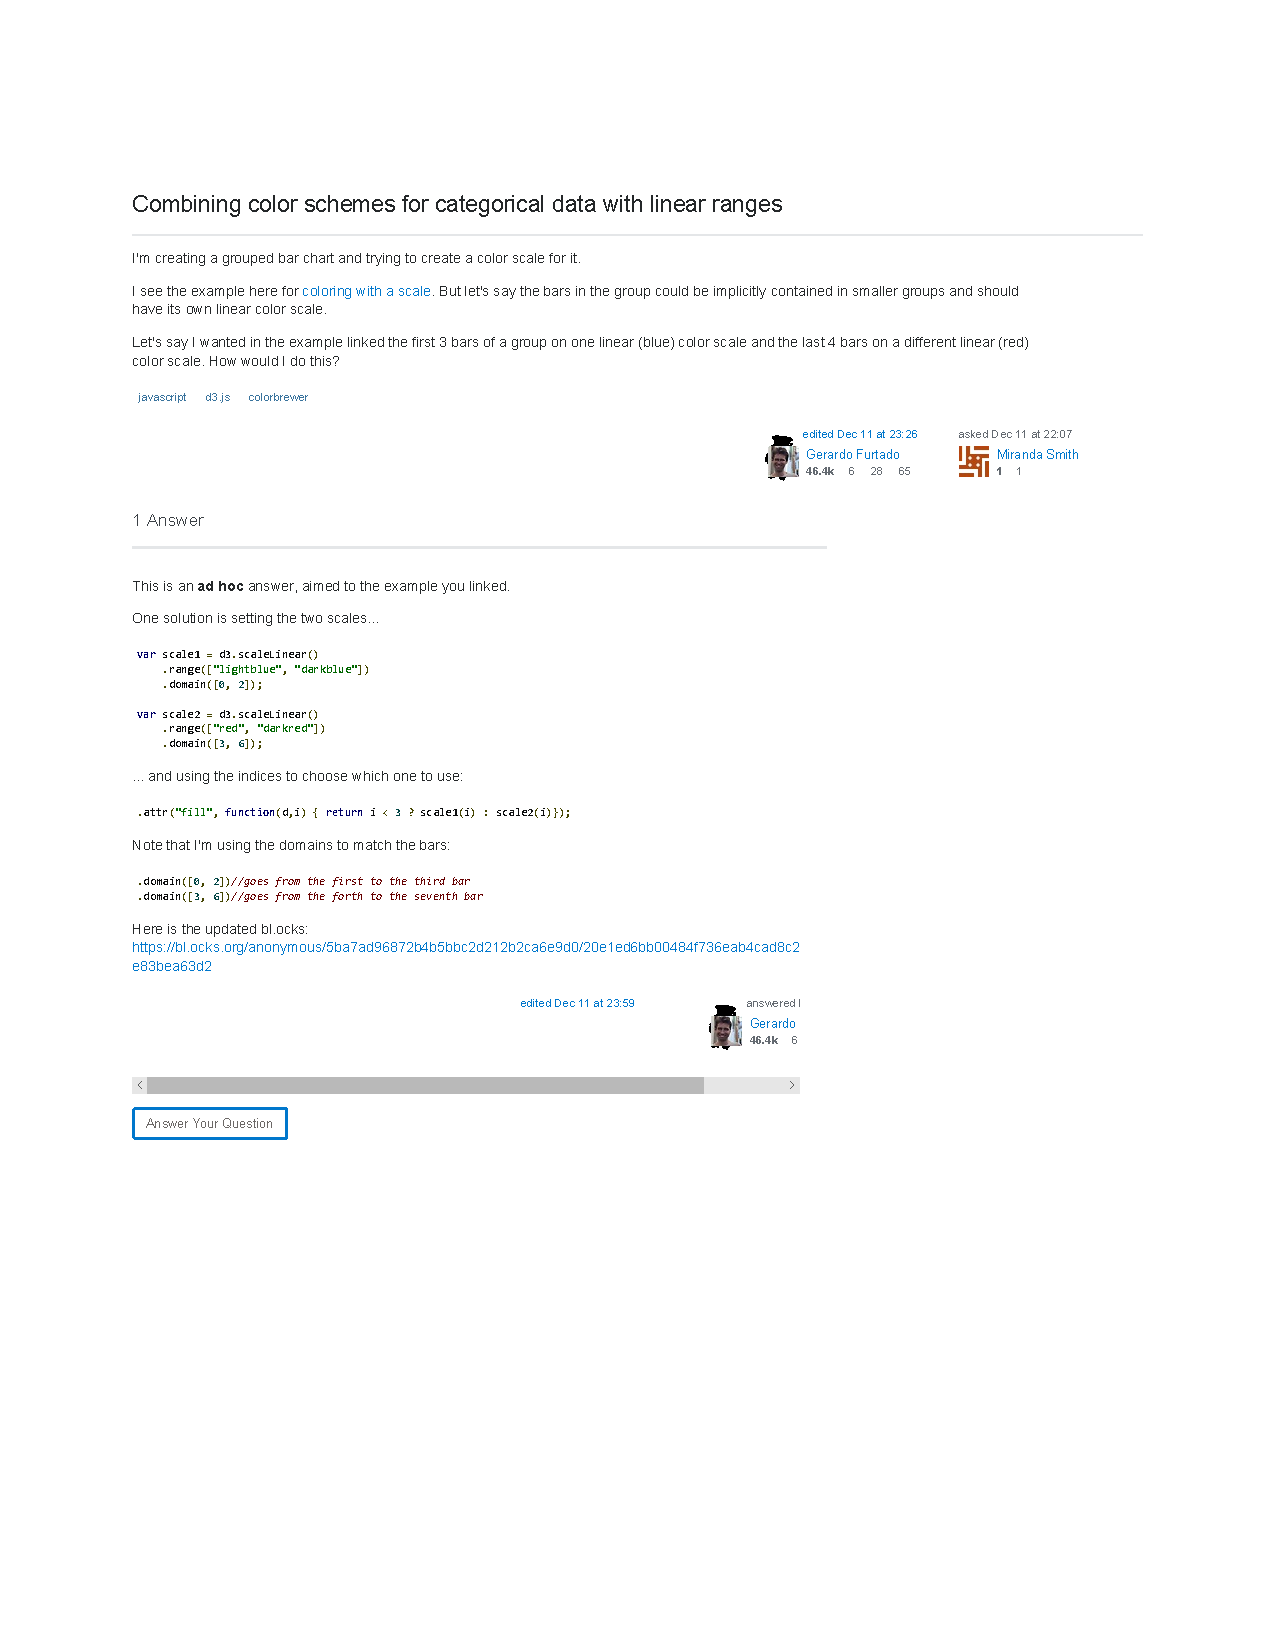
\includepdf[pages={1-}]{105lowquality.pdf}

I got one answer, and it was exactly what I had wanted and provided a better answer than I had found the first time I had to solve this question. They pointed out exactly what parts of the code to change and created a working example provided in a link to exactly what I was describing shown in Figure \ref{lowQ}. The effort seems to have been the same for both questions and provided well working high quality answers.

\begin{figure}[h]
  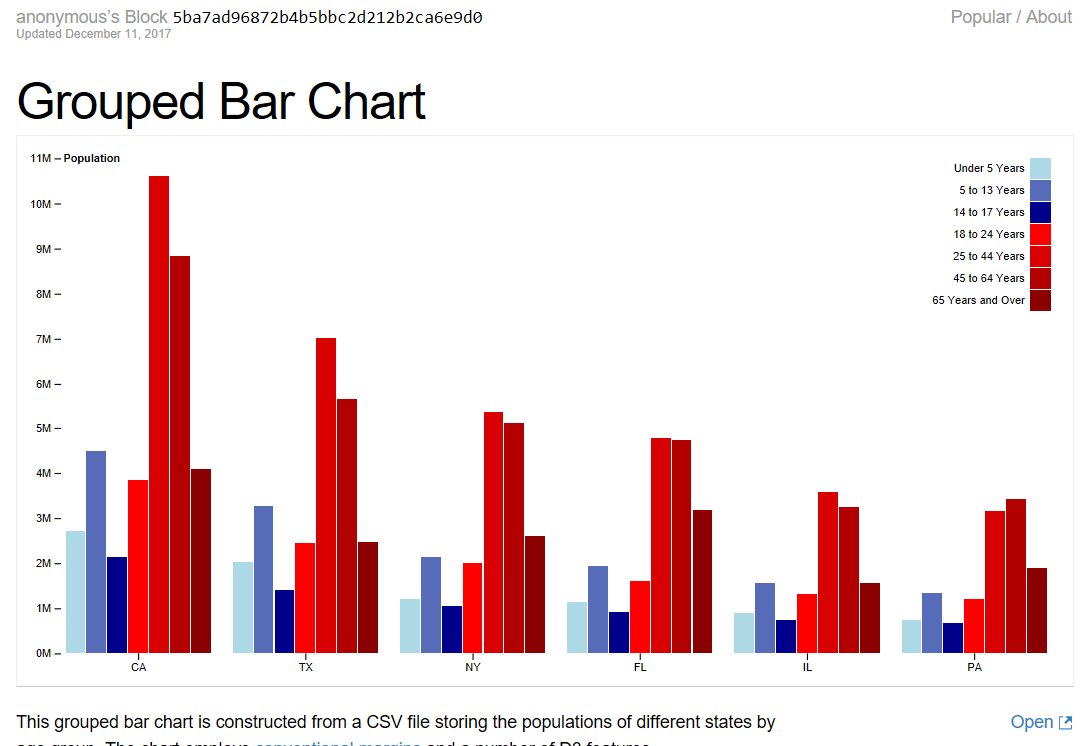
\includegraphics[width=\linewidth]{105answer.PNG}
  \caption{Solution Provided}
  \label{lowQ}
\end{figure}

\pagebreak

\section{Problem 10.6}
Find two examples of document filtering systems on the Web. How do they build a profile for your information need? Is the system static or adaptive?

\subsection{Solution}

The first example is \url{https://www.pinterest.com/}.  They build a profile for me by using an account and keeping track of what I like and pin to my own boards. The system is adaptive. I have been on pinterest for years and depending on what my most recent browsing history has been, pinterest shows me pins that relate most to recent interests.

The second example is \url{https://scholar.google.com/}. When I created a profile I created a filter for myself to send emails about articles I would be interested in based off a topic I specify. When I am logged in they also show recommended articles on the search screen. This system is static. It does not update based on interaction activity. If I wanted the content to change I would need to create another filter to replace it or add on to what I'm receiving. 

\section{Problem 10.11}
Suggest how the maximum and minimum resource ranking scores, Rmax and Rmin, could be estimated for a given query.

\subsection{Solution}
To get the Rmax for a particular resource that has been returned the resources need to be reordered so that the one in question has been returned first and recalculate the statistic that was used to order the resources. The same is true for Rmin except its position need to be the last possible position and still be returned. For example if the top 10 resources are being selected out of 100 returned then the position should be 10, not 100.

\pagebreak

\section{Problem 11.5}
How many papers dealing with term dependency can you find in the SIGIR proceedings since 2000? List their citations.

\subsection{Solution}

I queried google scholar for all papers matching the criteria "term dependency" OR "term dependent" OR "term dependence" source:SIGIR and it had to have been published in the range of 2000-2017. I got back 8 pages with 78 results. I downloaded Publish or Perish software\url{http://www.harzing.com/pop.htm} to download the results and scrape the pages for all the information I needed.


\begin{longtable}{|p{9cm}|p{5cm}|c|}

\hline
Title & Venue & Citations\\
\hline\hline
Incorporating term dependency in the DFR framework & … international ACM SIGIR … & 56  \\ \hline
Exploiting term dependence while handling negation in medical search & … international ACM SIGIR … & 21  \\ \hline
Score-safe term-dependency processing with hybrid indexes & … of the 37th international ACM SIGIR … & 10  \\ \hline
Modelling term dependence with copulas & … of the 38th international ACM SIGIR … & 8  \\ \hline
Parameterized fielded term dependence models for ad-hoc entity retrieval from knowledge graph & … of the 39th International ACM SIGIR … & 10  \\ \hline
Non-compositional term dependence for information retrieval & … International ACM SIGIR … & 7  \\ \hline
Utilizing phrase based semantic information for term dependency & … of the 31st annual international ACM SIGIR … & 0  \\ \hline
Improving Search using Proximity-Based Statistics & … 38th International ACM SIGIR Conference on Research … & 1  \\ \hline
Introduction to probabilistic models in IR & … 33rd international ACM SIGIR conference on Research … & 5  \\ \hline
A comparison of various approaches for using probabilistic dependencies in language modeling & … of the 26th annual international ACM SIGIR … & 16  \\ \hline
Two-stage query segmentation for information retrieval & … of the 32nd international ACM SIGIR … & 49  \\ \hline
Refining term weights of documents using term dependencies & … of the 27th annual international ACM SIGIR … & 9  \\ \hline
Query performance prediction in web search environments & … of the 30th annual international ACM SIGIR … & 169  \\ \hline
MRF based approach for sentence retrieval & … annual international ACM SIGIR … & 6  \\ \hline
Integrating word relationships into language models & … of the 28th annual international ACM SIGIR … & 184  \\ \hline
Building and applying a concept hierarchy representation of a user profile & … 26th annual international ACM SIGIR … & 80  \\ \hline
A Markov random field model for term dependencies & … of the 28th annual international ACM SIGIR … & 776  \\ \hline
Learning to efficiently rank & … of the 33rd international ACM SIGIR … & 74  \\ \hline
A study of Poisson query generation model for information retrieval & … of the 30th annual international ACM SIGIR … & 52  \\ \hline
Automatic P hrase Indexing for Document Retrieval: An Examination of Syntactic and Non-Syntactic Methods & ACM SIGIR Forum & 169  \\ \hline
Random walk term weighting for information retrieval & … of the 30th annual international ACM SIGIR … & 35  \\ \hline
Social annotation in query expansion: a machine learning approach & … of the 34th international ACM SIGIR … & 39  \\ \hline
Latent concept expansion using markov random fields & … of the 30th annual international ACM SIGIR … & 226  \\ \hline
Combining concepts and language models for information access & SIGIR Forum & 5  \\ \hline
A proximity language model for information retrieval & Proceedings of the 32nd international ACM SIGIR … & 69  \\ \hline
Learning to reweight terms with distributed representations & Proceedings of the 38th International ACM SIGIR … & 35  \\ \hline
Building a web test collection using social media & Proceedings of the 36th international ACM SIGIR … & 3  \\ \hline
Structured retrieval for question answering & … international ACM SIGIR … & 106  \\ \hline
An exploration of proximity measures in information retrieval & … of the 30th annual international ACM SIGIR … & 245  \\ \hline
Positional language models for information retrieval & Proceedings of the 32nd international ACM SIGIR … & 198  \\ \hline
Intent-aware search result diversification & … of the 34th international ACM SIGIR … & 98  \\ \hline
Sigir 2014 workshop on semantic matching in information retrieval & … of the 37th international ACM SIGIR … & 4  \\ \hline
Flat vs. hierarchical phrase-based translation models for cross-language information retrieval & … 36th international ACM SIGIR conference on Research … & 3  \\ \hline
Incorporating query term dependencies in language models for document retrieval & … of the 26th annual international ACM SIGIR … & 19  \\ \hline
Fielded sequential dependence model for ad-hoc entity retrieval in the web of data & … of the 38th International ACM SIGIR … & 33  \\ \hline
Dependence language model for information retrieval & … of the 27th annual international ACM SIGIR … & 294  \\ \hline
Axiomatic analysis for improving the log-logistic feedback model & … International ACM SIGIR … & 8  \\ \hline
Efficient \& Effective Selective Query Rewriting with Efficiency Predictions & … of the 40th International ACM SIGIR … & 0  \\ \hline
Query term ranking based on dependency parsing of verbose queries & Proceedings of the 33rd international ACM SIGIR … & 28  \\ \hline
CRTER: using cross terms to enhance probabilistic information retrieval & … of the 34th international ACM SIGIR … & 32  \\ \hline
Term Proximity Constraints for Pseudo-Relevance Feedback & … International ACM SIGIR … & 0  \\ \hline
Modeling higher-order term dependencies in information retrieval using query hypergraphs & … of the 35th international ACM SIGIR conference … & 54  \\ \hline
Topic-based index partitions for efficient and effective selective search & SIGIR 2010 Workshop on Large-Scale … & 16  \\ \hline
Building simulated queries for known-item topics: an analysis using six european languages & … 30th annual international ACM SIGIR … & 97  \\ \hline
Dynamic Factual Summaries for Entity Cards & Proc. of SIGIR & 2  \\ \hline
Set-based model: A new approach for information retrieval & … international ACM SIGIR … & 38  \\ \hline
Query term ranking based on search results overlap & … of the 34th international ACM SIGIR … & 1  \\ \hline
Exploiting proximity feature in bigram language model for information retrieval & … the 31st annual international ACM SIGIR … & 6  \\ \hline
Exploiting semantics for improving clinical information retrieval & … the 36th international ACM SIGIR … & 21  \\ \hline
A frequency-based and a poisson-based definition of the probability of being informative & … of the 26th annual international ACM SIGIR … & 39  \\ \hline
Efficient cost-aware cascade ranking in multi-stage retrieval & … International ACM SIGIR … & 3  \\ \hline
An adaptive evidence weighting method for medical record search & Proceedings of the 36th international ACM SIGIR … & 14  \\ \hline
Using key concepts in a translation model for retrieval & Proceedings of the 38th International ACM SIGIR … & 8  \\ \hline
Understanding negation and family history to improve clinical information retrieval & … of the 37th international ACM SIGIR conference … & 6  \\ \hline
Nordlys: A Toolkit for Entity-Oriented and Semantic Search & … 40th International ACM SIGIR … & 0  \\ \hline
Exploring reductions for long web queries & … international ACM SIGIR … & 74  \\ \hline
Learning for search result diversification & … the 37th international ACM SIGIR … & 42  \\ \hline
Color retrieval in vector space model & … ACM SIGIR Workshop … & 12  \\ \hline
Compact query term selection using topically related text & Proceedings of the 36th international ACM SIGIR … & 38  \\ \hline
DBpedia-Entity v2: A Test Collection for Entity Search & … ACM SIGIR … & 1  \\ \hline
Embedding-based Query Expansion for Weighted Sequential Dependence Retrieval Model & … of the 40th International ACM SIGIR … & 0  \\ \hline
On the cost of phrase-based ranking & Proceedings of the 38th International ACM SIGIR … & 1  \\ \hline
Extending BM25 with multiple query operators & Proceedings of the 35th international ACM SIGIR … & 14  \\ \hline
Learning for Efficient Supervised Query Expansion via Two-stage Feature Selection & … of the 39th International ACM SIGIR … & 2  \\ \hline
Parameterized concept weighting in verbose queries & … of the 34th international ACM SIGIR … & 100  \\ \hline
Diversity by proportionality: an election-based approach to search result diversification & Proceedings of the 35th international ACM SIGIR … & 93  \\ \hline
Paradox-free formal foundation of vector-space model & … of the ACM SIGIR 2002 workshop on … & 4  \\ \hline
Efficient in-memory top-k document retrieval & … of the 35th international ACM SIGIR … & 35  \\ \hline
Copulas for information retrieval & … international ACM SIGIR … & 19  \\ \hline
Automatic refinement of patent queries using concept importance predictors & … international ACM SIGIR … & 34  \\ \hline
Modeling Document Novelty with Neural Tensor Network for Search Result Diversification & … of the 39th International ACM SIGIR … & 10  \\ \hline
Term level search result diversification & Proceedings of the 36th international ACM SIGIR … & 36  \\ \hline
Learning user reformulation behavior for query auto-completion & … the 37th international ACM SIGIR … & 40  \\ \hline
A Probabilistic Model for Information Retrieval Based on Maximum Value Distribution & … 38th International ACM SIGIR Conference on Research … & 3  \\ \hline
Enhancing ad-hoc relevance weighting using probability density estimation & … of the 34th international ACM SIGIR … & 9  \\ \hline
Pseudo test collections for training and tuning microblog rankers & … international ACM SIGIR … & 17  \\ \hline
Introduction to Probabilistic Models for Information Retrieval & … of the 33rd International ACM SIGIR … & 4  \\ \hline
MEmbER: Max-Margin Based Embeddings for Entity Retrieval & … the 40th International ACM SIGIR … & 1  \\ \hline
\hline
\end{longtable}



\end{document}